\section{Microphone modules (small \& large)}
\begin{figure}[H]
    \centering
    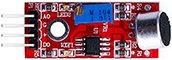
\includegraphics[angle=0, keepaspectratio=true, scale=1, width=200px, height=200px]{images/microphone_large.jpg}
    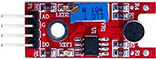
\includegraphics[angle=0, keepaspectratio=true, scale=1, width=200px, height=200px]{images/microphone_small.jpg}
    %\caption{Caption}
\end{figure}
\subsection*{Description}
The microphone modules have both an analog and digital output. When the microphone detects sound the analog output of the module will be proportional to the loudness of the sound. Also if the loudness is above a certain threshold the digital output of the module is set to high.

The microphone is not particularly sensitive, so you may need to blow into the microphone from a close range for it to detect any sound.

\subsection*{Pin mapping}
This pin mapping corresponds to the pins from left to right with the module pins facing towards you.
\begin{table}[H]
    \centering
    \begin{tabular}{|c|c|c|c|c|}
    \hline
    Index &Label &Type &Name &Description\\ \hline
    0 &A0 &Analog output &A0 &Signal to activate relay \\ \hline
    1 &G &Ground &GND &\\ \hline
    2 &+ &Source voltage &$V+$ &Module source voltage ($5V$)\\ \hline
    3 &D0 &Digital output &D0 &\\ \hline
    \end{tabular}
    %\caption{Caption}
    %\label{tab:my_label}
\end{table}
\subsection*{Operation}
The output voltage at the analog pin (A0) is related to the loudness of the sound detected by the microphone.

The output voltage at the digital pin (D0) is set to high when microphone detects a sound louder than a set threshold. This threshold can be set by adjusting the potentiometer on the module.

%\lstinputlisting[caption=test]{laser.py}